\documentclass[a4paper,12pt]{article} 
\usepackage[T2A]{fontenc}			
\usepackage[utf8]{inputenc}			
\usepackage[english,russian]{babel}	
\usepackage{amsmath,amsfonts,amssymb,amsthm,mathtools} 
\usepackage[colorlinks, linkcolor = blue]{hyperref}
\usepackage{upgreek}\usepackage[left=2cm,right=2cm,top=2cm,bottom=3cm,bindingoffset=0cm]{geometry}
\usepackage{graphicx}
\usepackage{xcolor}
\author{Дорогинин Д.В.}
\title{3.3.4. Эффект Холла в полупроводниках.}
\date{\today}
\begin{document}
\maketitle
\newpage
\textbf{Цель работы}: измерение подвижности и концентрации носителей заряда в полупроводниках.


\textbf{В работе используются}: электромагнит с источником питания, амперметр, милливеберметр, реостат, источник питания, цифровой вольтметр, образцы легированного германия.\\
\section*{Описание работы}
\begin{center}
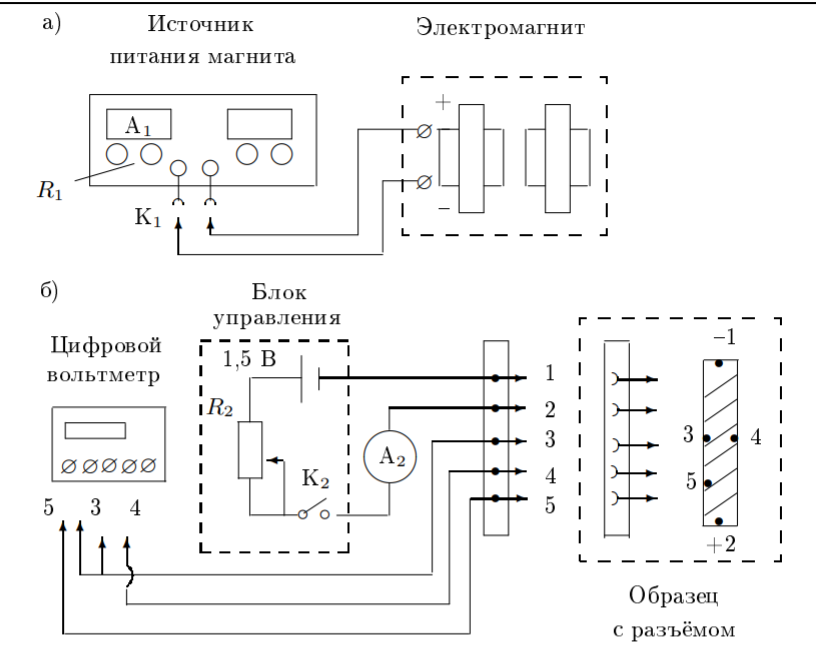
\includegraphics[scale=0.5]{1.png}
\end{center}
Схема для измерения ЭДС Холла представлена на рисунке. В зазоре электромагнита создаётся постоянное магнитное поле, величину которого можно менять регуляторами источника питания электромагнита. Градуировка магнита проводится при помощи милливеберметра.\\
Образец из легированного германия, смонтированный в специальном держателе, подключается к источнику питания. При замыкании К$_2$ вдоль длинной стороны образца течёт ток, величина которого регулируется реостатом $R$ и измеряется миллиамперметром. В образце, помещённом в зазор, возникает разность потенциалов $U_{34}$, которая измеряется с помощью цифрового вольтметра.\\
Влияние омического падения напряжения исключается измерением напряжения $U_0$ между 3 и 4 в отсутствие магнитного поля. По знаку $\mathcal{E} = U_{34} \pm U_0$ можно определить характер проводимости -- электронный или дырочный, зная напрявление тока в образце и напрвление магнитного поля.\\
Померив ток $I_{35}$ в образце и напряжение $U_{35}$ между контактами 3 и 5 в отсутствие магнитного поля можно рассчитать проводимость материала по формуле
$$
\sigma = \frac{IL_{35}}{U_{35}al},
$$
где $L_{35}$ -- расстояние между контактами 3 и 5, а $a$ и $l$ -- толщина и ширина образца.
\section*{Ход работы}
\begin{enumerate}
\item Подготовим установку к работе.
\item Проградуируем электромагнит. Определим связь между индукцией $B$ магнитного поля в зазоре электромагнита и током $I_M$ через обмотку сняв зависимость потока $\text{Ф} = BSN$, пронизывающего пробную катушку, находящуюся в зазоре, от тока $I_M$. Значение $SN = 72~\text{см}^2 \cdot \text{вит}$.
\begin{table}[h]
\centering
\begin{tabular}{|l|l|l|l|l|l|l|l|l|}
\hline
$I$, А  & 0.2   & 0.4   & 0.6  & 0.8   & 1     & 1.2   & 1.4   & 1.6  \\ \hline
$B$, Вб & 0.012 & 0.027 & 0.04 & 0.053 & 0.063 & 0.072 & 0.077 & 0.08 \\ \hline
\end{tabular}
\end{table}
\item Проведём измерение ЭДС Холла. Для этого вставим образец в зазор выключенного электромагнита и определим $U_0$ между контактами 3 и 4 при минимальном токе через образец.\\
Включим электромагнит и снимем зависимость $U_{34}=f\left(I_M\right)$ от тока $I_M$ при постоянном токе через образец в интервале $0.3-1.0$ мА. При максимальном токе также проведём измерения при другом направлении магнитного поля.
\begin{table}[h]
\centering
\begin{tabular}{|l||l||l|l|l|l|l|l|l|l|}
\hline
$I_M$, А & $U_0$, мкВ & \multicolumn{8}{l|}{$-U_{34}$, мкВ}  \\ \hline
30  & 8  & 9   & 29  & 52  & 74  & 93  & 106 & 116 & 123 \\ \hline
40  & 13 & 16  & 47  & 75  & 105 & 128 & 146 & 158 & 167 \\ \hline
50  & 15 & 22  & 62  & 98  & 134 & 162 & 187 & 201 & 209 \\ \hline
60  & 16 & 28  & 73  & 119 & 158 & 197 & 222 & 239 & 251 \\ \hline
70  & 18 & 34  & 85  & 137 & 187 & 229 & 263 & 283 & 298 \\ \hline
80  & 21 & 41  & 104 & 166 & 225 & 273 & 306 & 327 & 341 \\ \hline
90  & 23 & 41  & 111 & 177 & 243 & 298 & 327 & 366 & 382 \\ \hline
100 & 26 & 50  & 131 & 211 & 279 & 338 & 378 & 406 & 423 \\ \hline
100 & 45 & 131 & 205 & 282 & 353 & 412 & 453 & 483 & 500 \\ \hline
\end{tabular}
\end{table}
\item Определим знак носителей в образце. Узнаем направление тока в образце и в электромагните, с помощью последнего определим направление магнитного поля.
\item При токе $I = 1,00 \pm 0,02~\text{мА}$ измеряем падение напряжения между концами 3 и 5: $U_{35} = 1666 \pm 1~\text{мкВ} $. Характеристики образца: $L_{35} = 3~\text{мм}, a = 1.5~\text{мм}, l = 1.7~\text{мм}$.
\end{enumerate}
\section*{Обработка результатов}
\begin{enumerate}
\item Расчитаем индукцию магнитного поля $B$ для каждого значения тока и построим график $B = f(I_M)$.\\
\begin{center}
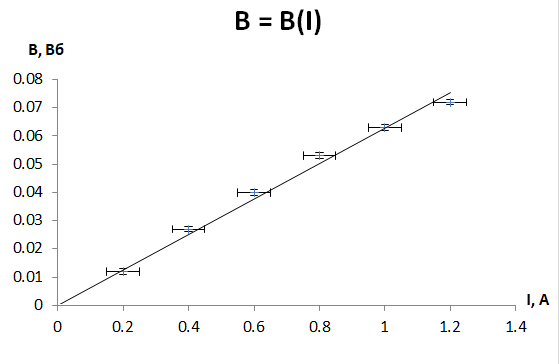
\includegraphics[scale=0.6]{4.png}
\end{center}
\item Рассчитаем ЭДС Холла и построим на одном графике семейство характеристик $\mathcal{E}_x=f(B)$ при разных токах, определим угловые коэффициенты $k(I)=\Delta \mathcal{E}/ \Delta B$.\\
\begin{center}
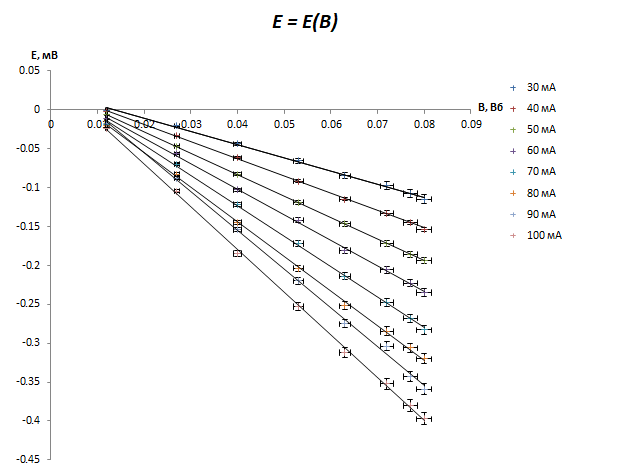
\includegraphics[scale=0.6]{2.png}
\end{center}
Построим график $k = f(I)$, рассчитаем угловой коэффициент и по формуле $\mathcal{E}_x= -R_x \cdot \frac{IB}{a}$ рассчитаем постоянную Холла $R_X$.
\begin{center}
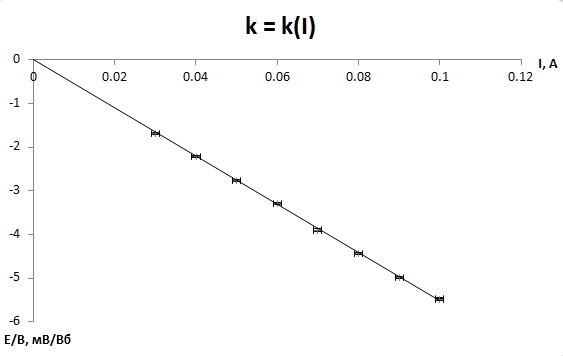
\includegraphics[scale=0.6]{3.png}
\end{center}
\begin{table}[h]
\centering
\begin{tabular}{|l|l|l|l|l|l|l|l|l|}
\hline
$k$, мВ/Вб  & -1.7 & -2.2 & -2.8 & -3.3 & -3.9 & -4.4 & -5.0 & -5.5 \\ \hline
$I_M$, А & 0.03  & 0.04  & 0.05  & 0.06  & 0.07 & 0.08  & 0.09  & 0.1   \\ \hline
\end{tabular}
\end{table}
$$
R_x=(83 \pm 1)\cdot 10^{-6} \frac{\text{м}^3}{\text{Кл}}.
$$
\item По формуле $R_x=\frac{1}{ne}$ рассчитаем концентрацию носителей тока в образце: $n = (750 \pm 9)\cdot 10^{20} \dfrac{1}{\text{м}^3}.$
\item По формуле $\sigma = \dfrac{IL_{35}}{U_{35}al}$ рассчитаем удельную проводимость материала образца: $\sigma = 706 \pm 1 \dfrac{1}{\text{Ом}\cdot\text{м}}$.
\item По формуле $b = \dfrac{\sigma}{en}=\sigma R_x$ вычислим подвижность носителей носителей тока в образце: $b = 0.060\pm 0.001 \dfrac{\text{м}^2}{B\cdot c}$.
\end{enumerate}
\end{document} 